\addcontentsline{toc}{section}{Repository for the code : R Package}
\section*{Repository for the code : R Package}

The created \textbf{R package} can be easily downloaded from this \href{https://github.com/proto4426/PissoortThesis}{\textbf{repository}} :
\begin{center}\label{xxx}
 \url{https://github.com/proto4426/PissoortThesis}
\end{center}
by following instructions in the README. It follows the standard structure of a usual R package (see e.g. \citet{leisch_creating_2008}) and makes use of the \texttt{roxygen2} package for the documentation.

For the reader's convenience, an external folder has been created in the above repository containing all the scripts created during this thesis. It allows reproduction of the results often with more details, tables or plots. It is located in the \textbf{/Scripts-R/} folder of the repository. Each script will be mentionned in its corresponding section. Further details on the repository structure can be found in \hyperref[appgit]{Appendix \textbf{\ref{appgit}}}.

\addcontentsline{toc}{subsection}{Visualization Tool : Shiny Application}
\subsection*{Visualization Tool : Shiny Application}

Shiny applications that have been developed can be run directly through the R environment after loading the package in your environment, by executing 

\begin{center}
\begin{lstlisting}[language=R]
runExample()  # in the R console,
\end{lstlisting}
\end{center}
choosing one applications's name between the displayed propositions and write it inside (' ').
So far, we have
\begin{itemize}
	\item[-]('GEV\_distributions') :  application based on Figure \ref{gevdens} smoothly displaying the GEV and the influence of its parameters.
	
	\item[-] ('trend\_models') :
	application dedicated to annual maxima that can be visualized with some preliminary methods (see \hyperref[sec:firstvisu]{Section \textbf{\ref{sec:firstvisu}}}).
	
	\item[-] ('splines\_draws') : application that simulates splines of a GAM model to visualize the difference in coverages between pointwise and simultaneous confidence intervals. (see \hyperref[sec:splines]{Section \textbf{\ref{sec:splines}}}).

	\item[-] ('neural\_networks') : 
	application for \texttt{GEVcdn} allowing bagging to demonstrate the effects of all the (hyper)parameters, since these choices can be subjective...
\end{itemize}
A dynamic overview of the applications is available in the repository's \texttt{README}.

\paragraph*{All-in-one : Dashboard} 
Still for the reader's convenience, all applications have been placed in a smooth \emph{dahsboard}. Moreover, it is uploaded on a server at the following \href{https://proto4426.shinyapps.io/All\_dashboard/}{URL}\footnote{\url{https://proto4426.shinyapps.io/All\_dashboard/}}
 in order to provide a quick user-friendly overview through the \texttt{rsconnect} interface.
 
The rest of the analysis in this chapter will rely on \texttt{1intro\_stationary.R} and \\ \texttt{1intro\_trends(splines).R} codes from the \textbf{/Scripts-R/} folder of the \href{https://github.com/proto4426/PissoortThesis}{repository}.


\section{Presentation of the Analysis : Temperatures from Uccle}\label{sec:presuccle}

Data used in this thesis comes from the "Institut Royal de Météorologie" (IRM) in Uccle in order to have reliable data provided by Belgian meteorologists.
IRM provided a set of databases this thesis focuses on temperature analysis in order to assess climate warming.% Rainfall data analysis would have also been interesting in EVT. 

The fact that the dataset begins only at year $1901$ is due to homogeneity reasons since the measurement shelters evolved substantially compared to previous periods, especially in terms of measurement errors. 
For meteorological considerations and again for reasons of homogeneity, it is better to analyze the temperatures in \emph{closed shelters}, following for example \citet{lindsey_use_1956}. Indeed, thanks to helpful advice from C.Tricot, climatologist at the IRM, temperatures in closed shelters have the advantage of not being overly influenced by solar radiation which artificially increases temperatures, especially in periods of extreme heats and high solar activity, and therefore in the studied case. 
For example, the maximum temperature of $36.6^{\circ}c$ that occurred on 27th June 1947 in closed shelters was measured at $38.8^{\circ}c$ in open shelters the same day.



\subsection*{Comparisons with freely available data} 

A similar dataset for Uccle is publicly available on the \href{http://lstat.kuleuven.be/Wiley/Data/ecad00045TX.txt}{Internet}\footnote{\url{http://lstat.kuleuven.be/Wiley/Data/ecad00045TX.txt}}. It was a project initially performed by the KMNI and which was used by \citet{beirlant_statistics_2006}. However, we did not want to analyze this data for reliability reasons as mentioned above.

Afterwards, we compared these two datasets for years $1901$ to $2001$. Note that there are large differences
in these two datasets. For example,
$54\%$ of measurements are equal with those of the dataset in open shelters against $14.4\%$ in the closed shelters. This gives confidence that the public dataset has temperatures measured in open shelters, which is not recommended. Hence, we conclude that large measurement errors can easily occur in unofficial data emphasizing the necessity of reliable data in order to yield a reliable analysis.

\section{First Analysis : Annual Maxima}\label{sec:firstana}


\subsection{Descriptive Analysis}

The goal of this section is to display a global overview of the data. The code provided most of the descriptive analysis. To summarize most of the information, we have plotted a violin-plot and a density plot of the \textbf{daily} maximum temperatures in Figure \ref{fig:violin_density} in \hyperref[app:fig]{Appendix \textbf{\ref{app:fig}}} where we divided data in each meteorological season to highlight the differences. For example, we can see that the spread is higher for autumn and spring.

We will use the block-maxima approach by taking yearly blocks leaving us with $n=116$ years of data, which seems justifiable for further GEV analysis and the convergence to hold. We will discuss the choice of the block length further in the \hyperref[sec:anagev]{next Chapter}.

\subsection{First visualization with simple models}\label{sec:firstvisu}

Below is the series of yearly maxima in Figure \ref{first_fig} where we introduce 3 \textbf{models for the trend} :


\begin{figure}[!htb]
	\centering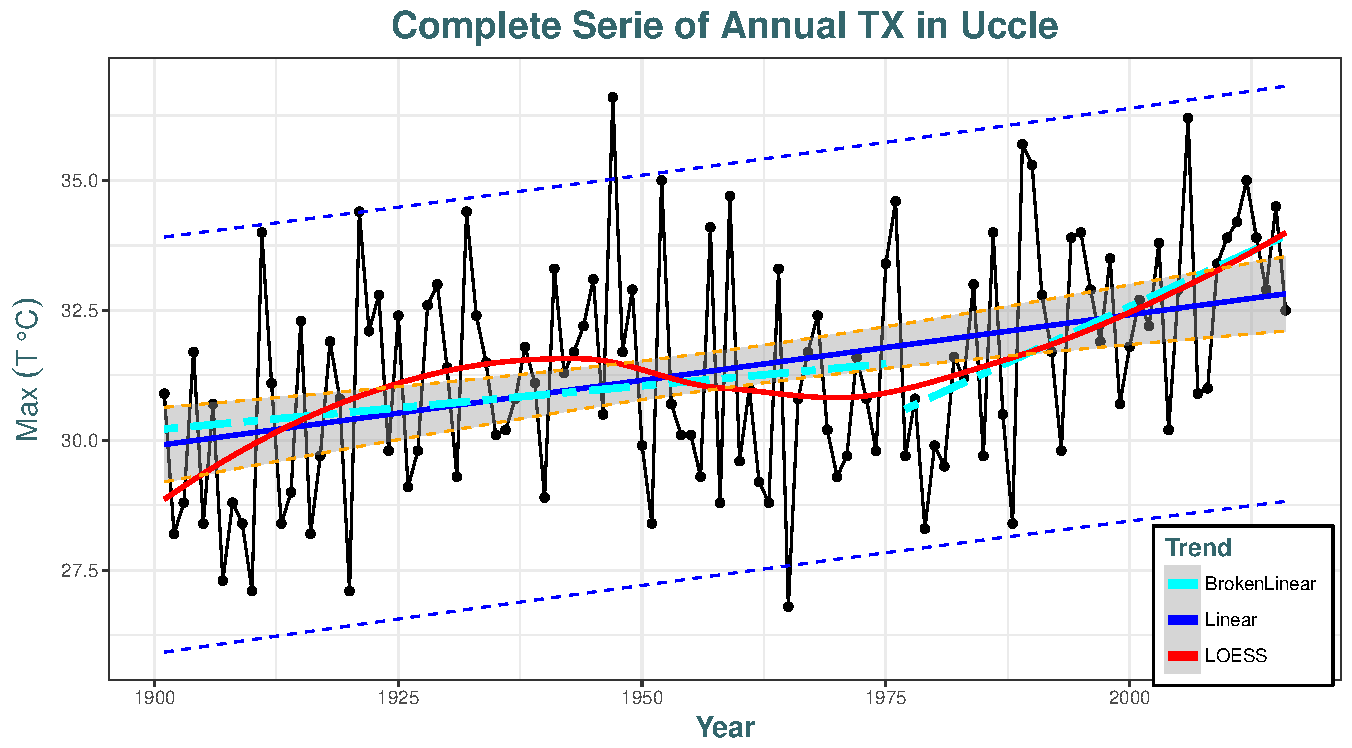
\includegraphics[width=.8\linewidth]{gg12.pdf}\caption{Yearly maxima together with three first models that represent the trend. Note the shaded grey area around the linear regression fit is $95\%$ pointwise confidence interval on the fitted values (i.e., $\pm 1.96\times \sigma_{pred}(\text{year})$) while blue dotted lines are prediction intervals taking into account the prediction uncertainty.}%i.e. there is $95\%$ confidence that the "true" (population) regression line lies within the shaded region.}
\label{first_fig}
\end{figure}


\begin{itemize}
\item \emph{Linear regression} is a \textbf{parametric} fit. Note that it is slightly but significantly increasing over time ($\text{p-value}\approx 10^{-5}$). From this model, one rough deduction is that each year we expect the annual maximum temperature to increase by $\hat{b}=0.025^{\circ}c$ \  (with $\hat{\sigma}_{\hat{b}}=0.005)$.

\item \emph{Local Polynomial regression } or LOESS is a \textbf{nonparametric} fit which smooth the data. The drop in the series visible around years $1950$ to $1975$ is probably due to noise rather than a real decrease or freezing of the maximum temperatures. Moreover, it disappears if we change the parameter controlling the degree of smoothing. We will assess that more formally in the \hyperref[sec:splines]{next Section} with another nonparametric model.

\item \emph{Broken-linear regression} is a \textbf{parametric} fit. We wanted to emphasize visually the trend difference between the period [1901-1975] and [1976-2016]. These two periods have been chosen arbitrarily and we note that period [1901-1952] has also a very high positive slope. We will study that in more details in the \hyperref[sec:splines]{next Section}.
\end{itemize}
These different models give us insights on the process we will study throughout the rest of this thesis. We will not develop further the results of each model as this is not the aim of this thesis rather we are interested in assessing the trend and its statistical significance over time using more sophisticated methods.


\subsection{Deeper Trend Analysis : Splines derivatives in GAM}\label{sec:splines}

Apart from the significant pointwise increasing linear trend, we did not find concrete results. Additionally, we see in the series in Figure \ref{first_fig} that a linear trend to the entire series could be too restrictive. The LOESS or the broken-linear trend highlight that the trend is not constant over time.
We would like here to assess more formally this difference in the slope of the trend over time. 

This section assumes reader knowledge of \emph{Generalized Additive Models} (GAM) developed by \citet{hastie_generalized_1986} and on \emph{penalized splines}. Theoretical explanations of these concepts can be found in \citet[chapter 3, 6 and 11]{ruppert_semiparametric_2003}, the reference book of this section. Replacing covariates with smooth functions such as smoothing splines will result in a more flexible nonparametric model. We will also follow the simulation-based Bayesian approach of \citet{marra_coverage_2012} that compares coverage properties of intervals.


\addcontentsline{toc}{subsubsection}{Pointwise vs Simultaneous intervals}
\subsubsection*{Pointwise or Simultaneous confidence intervals ?}

For this analysis, we deem important to differentiate the two types of intervals for a better understanding of the actual meaning of "confidence interval". A special example is the grey area around the linear fit in Figure \ref{first_fig} which represents a $95\%$ interval for the regression line, taking into account only variability in the data. For instance, if we repeatedly sample and take the predicted values, then the new linear fit will be in the grey zone approximately $95\%$ of the time.

Let $\mathcal{X}$ denote the set of $x$ values of interest, i.e. $\mathcal{X}=[1901,2016]$ in our case and $f(\cdot)$ is the model of interest, e.g. the linear regression, or the GAM model that we will fit. Hence, we define 
\begin{itemize}
	\item A \textbf{pointwise} $100(1-\alpha)\%$ confidence interval $\Big\{\big[L(x),U(x)\big] \ : \ x\in \mathcal{X}\Big\}$ approximately satisfies
	\begin{equation}
	\text{Pr}\Big\{L(x)\leq f(x)\leq U(x)\Big\}\geq 1-\alpha, \qquad \forall x\in\mathcal{X}.
	\end{equation}
	
	\item A \textbf{Simultaneous} $100(1-\alpha)\%$ confidence interval must satisfy 
	\begin{equation}
	\text{Pr}\Big\{L(x)\leq f(x)\leq U(x), \ \forall x\in\mathcal{X}\Big\}\geq 1-\alpha.
	\end{equation}
\end{itemize} 
In the linear regression example of Figure \ref{first_fig}, from the pointwise confidence intervals we can say that, $f(1920)$ has $95\%$ chance to lie within $[29.8,\ 31.1$] and $f(2016)$ has also $95\%$ to lie within $[32.1, \ 33.6]$ but it would be false to say that both are contained in these intervals at the same time with $95\%$ confidence. The corresponding simultaneous intervals (blue dotted lines) are quite larger, $[26.4, \ 34.3]$ and $[36.8, \ 28.8]$ for years $1920$ and $2016$ respectively.
For the interested reader, theoretical details on how to mathematically derive simultaneous intervals are available in \citet[pp.142-144]{ruppert_semiparametric_2003}.


\addcontentsline{toc}{subsubsection}{Methodology}
\subsubsection*{Methodology}

\begin{itemize}
\item We have fitted a GAM model on the annual maxima relying on the \texttt{mgcv} package from \citet{maindonald_data_2006}.

\item  Figure \ref{fig:acfresgam1} in \hyperref[app:fig]{Appendix \textbf{\ref{app:fig}}} shows the correlation structure of the serial normalized residuals. As the selection of a model for the residuals is not trivial from this figure, we fitted several time series models for the residuals. It is not necessary to consider too complex models, therefore 2 additional degrees of freedom are sufficient. Results are in Table \ref{table:gamresid} in \hyperref[app:fig]{Appendix \textbf{\ref{app:fig}}} where we see that BIC will prefer the independent model for the residuals but the AIC will not. Parsimony being important, we chose the independent model to draw plots with simultaneous intervals but we will also keep MA(1) for comparisons. Likelihood ratio tests validated our choice. Diagnostics of the model presented in Figure \ref{fig:diagnogam} in \hyperref[app:fig]{Appendix \textbf{\ref{app:fig}}} are correct.

\item As we took a Gaussian (identity) link, our model can hence be written as

\begin{equation}\label{eq:gam}
Y_{\text{GAM}}(\text{year}) = \alpha + f_{\text{(k)}}(\text{year})+\epsilon , \qquad\quad \epsilon\sim\text{WN}.
\end{equation}
where $f$ is modelled by smoothing splines, $\epsilon$ can be MA(1) and $Y$ represent annual TX. We set the dimension of the basis $k$ for the spline to $20$ to ensure a reasonable degree of smoothness as there is modest amount of non-linearity in the series and we did not perform cross-validation as it will not influence the results significantly. 

\item  To account for uncertainty, we simulated $M = 10^4$ draws (quite fast) from the posterior of the GAM model in (\ref{eq:gam}). Hence, the confidence intervals (or bands) that we compute will be of the form of Bayesian credible intervals,  discussed in \hyperref[bayes_cred_int]{Section \textbf{\ref{bayes_cred_int}}} and which is highlighted by \citet{marra_coverage_2012}.
$50$ posterior draws are displayed in Figure \ref{fig:post_draws} %let in \hyperref[app:fig]{appendix \ref{app:fig}}
 displaying pointwise (in yellow) and simultaneous (in red) intervals. We point out that pointwise intervals are too narrow.
\end{itemize}

\begin{figure}[!htb]
	\centering	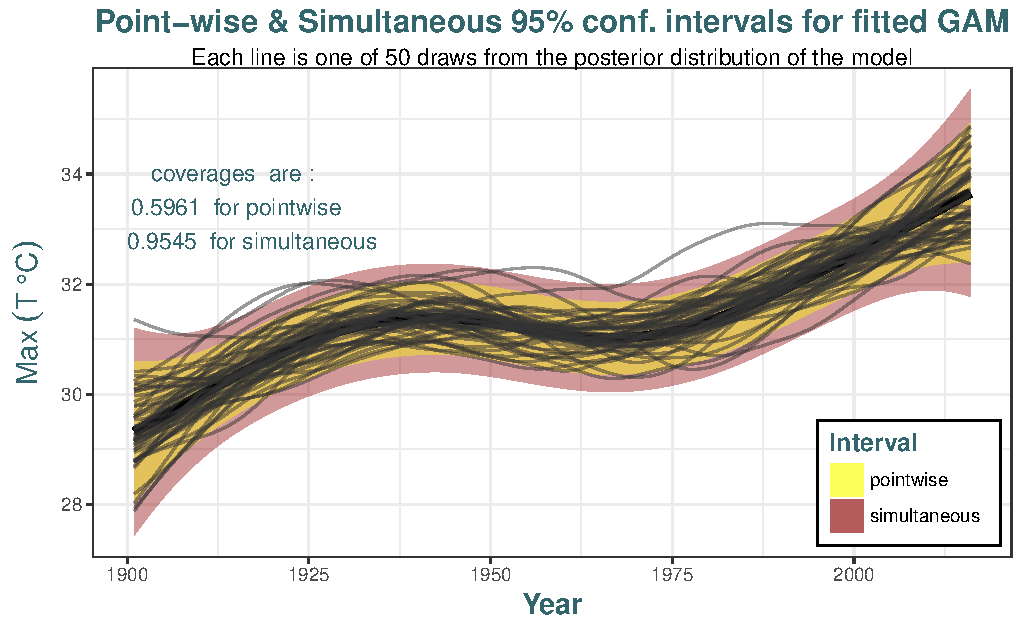
\includegraphics[width=.75\linewidth]{post_draws.pdf}\caption{Draws from the posterior distribution of the model. Notice the large uncertainty associated to the posterior draws (grey lines).  The coverages are calculated for $M=10^4$ simulations. }\label{fig:post_draws}
\end{figure}

\subsubsection*{Coverage Analysis} 

To highlight the inadequacy of the pointwise intervals, we computed posterior draws of the fitted GAM and we counted how many draws lied within each interval.

\begin{table}[!htbp] \centering 
  \caption{Proportion of the $M$ posterior simulations which are covered by the confidence intervals} \label{tab:cov} 
\begin{tabular}{@{\extracolsep{5pt}}lccccc} 
\toprule	
\vspace{-.1cm}\\[-1.8ex] 
\textbf{Coverage at $95\%$} & \multicolumn{1}{c}{$M=20$} &  \multicolumn{1}{c}{$M=100$} & \multicolumn{1}{c}{$M=10^3$} & \multicolumn{1}{c}{$M=10^5$} \vspace{.1cm} \\ 
\midrule	
\underline{Pointwise} & $40\%$ & $63\%$ & $61.1\%$ & $59.463\%$ \\
\underline{Simultaneous} & $80\%$ & $91\%$ & $94.9\%$ & $95.019\%$  \\
\bottomrule	
\end{tabular} 
\end{table}
We can see that the coverages converge to the true value $95\%$ of the confidence level for the simultaneous intervals when $M$ becomes very large, while it converges to $\approx 60\%$ for the pointwise intervals.

Shiny application has been build from this graph for better visualization of the impact of the number of simulations on the confidence intervals and how coverage varies, both visually and quantitatively.
Finally, note that the results are similar if we do the experiment on the first derivatives $f^{'}(\cdot)$ of the splines rather than on the splines themselves.


\addcontentsline{toc}{subsubsection}{Final Results}
\subsubsection*{Final Results}

We see two significant increases in the trend fitted by GAM in Figure \ref{fig:center_gam} in \hyperref[app:fig]{Appendix \textbf{\ref{app:fig}}} when we do not use  simultaneous intervals. The decrease pointed out in Figure \ref{first_fig} with LOESS between $1945$ and $1970$ is hence not significant and probably due to randomness.

Some remarks from the two plots in Figure \ref{fig:derivsplines}, considering now splines derivatives :

\begin{figure}[!htb]
	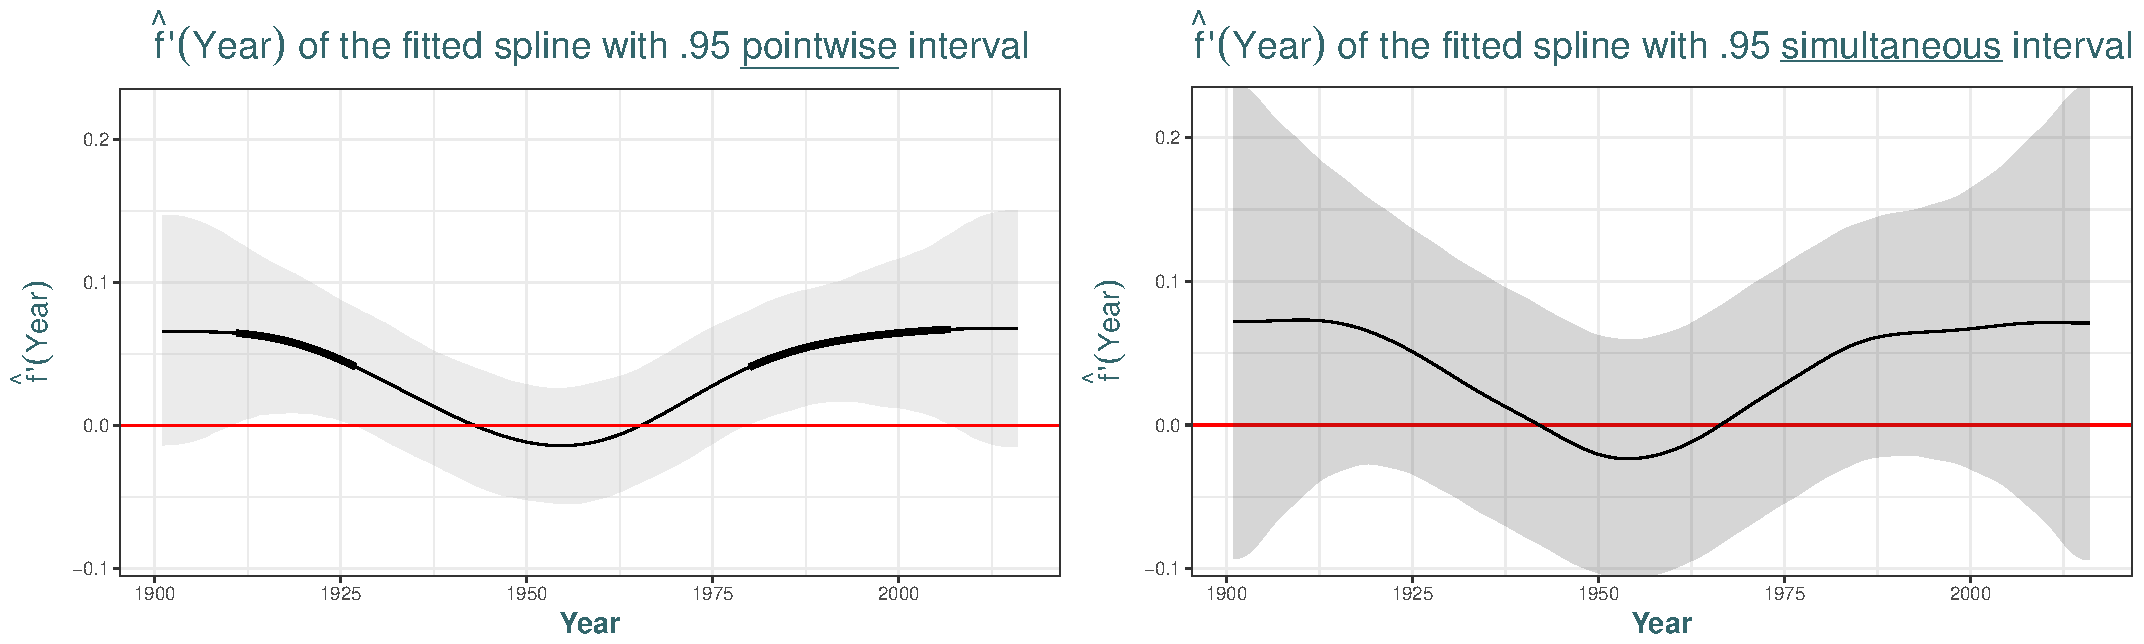
\includegraphics[width=.99\linewidth]{splines.pdf}\caption{Plots of the first derivative $f_{(20)}^{'}(\text{year})$ of the estimated splines on the retained GAM model. Grey area represents $95\%$ confidence bands. Sections of the spline where the confidence interval does not include zero are indicated by thicker lines. }\label{fig:derivsplines}
\end{figure}

\begin{itemize}
\item Together with the series in Figure \ref{first_fig}, we can make the link between the trend behavior of the series and the splines' first derivatives which accurately models the slope behavior of the trend. 
\item Note the increasing trend with decreasing slope, i.e. $ f_{(20)}^{''}(\text{year})<0$, until year $\approx 1945$ where it becomes negative. The slope then increases and the trend starts to increase again near 1962. This upward trend in the series of annual maxima for this last period brings light to the climate change we are currently facing. However, we see that we are now at a "critical point" for several years, i.e. $f_{(20)}^{''}(\text{year})\approx 0$, meaning that the trend is likely linear. 

\item  Whilst the pointwise confidence interval includes significant regions, i.e. 0 is not included in the interval, the simultaneous interval that is accounting for the increase in uncertainty has no significant regions. Therefore, we cannot conclude that there has been any significant increase in the annual maximum temperatures in any period.

\end{itemize}


\section{Comments and Structure of the Analysis }

 We have found that there is an upward (linear) trend for the series of yearly maxima, but it is not significant once corrected for simultaneous intervals.
Hence, a nonstationary analysis is worth continuing with.
After this introductory analysis, we will continue with the specific subject of this thesis, the extreme value analysis. Hence, \hyperref[sec:anagev]{next Chapter} will present a stationary GEV analysis and then allow nonstationarity in various ways. Bayesian analysis will finally try to make additional improvements in \hyperref[sec:anabayes]{Chapter \textbf{\ref{sec:anabayes}}}, e.g. with quantification of uncertainty or in computational efficiency.


As you have seen, the analysis in POT or in GEV involves different methods and different subsets of data. In this text, we will not display the results of the POT analysis for ease of reading. Henceforth, we will focus on the GEV analysis only. Note that the POT analysis is available on the \href{https://github.com/proto4426/PissoortThesis}{repository} presented above (or see
\hyperref[appgit]{Appendix\textbf{ \ref{appgit}}}).


Moreover, we have also conducted some analysis by dividing the dataset by seasons, by hot or cold months (July-August or January-February), etc. We have also analyzed annual minimum temperatures and found a less pronounced trend than for maxima.
Interesting comparisons are also available on the \href{https://github.com/proto4426/PissoortThesis}{repository}, but this text will focus on a GEV analysis on yearly maxima.